\documentclass[11pt,oneside,a4paper]{article}
%\usepackage{ucs}
\usepackage{url}
\usepackage{hyperref}
\usepackage[pdftex]{graphicx}
\usepackage{textcomp}
\usepackage[latin1]{inputenc}
\usepackage[finnish]{babel}
\usepackage[T1]{fontenc}
\author{Jari Koskinen, Hansi Keijonen, Eero Laine}
\title{Ohjelmointikielten periaatteet 2013} 




\begin{document}
% kirjoita nimi�
\maketitle

\pagebreak

\tableofcontents

\pagebreak

\section{D ohjelmointikieli}
D on kehitetty korjaamaan C ja C++ kielten puutteita ja samalla siihen on lis�tty paljon ominaisuuksia, joiden ansiosta...
\subsection{Yleist�}
D kieless� on ominaisuuksia plaaplaa...
\begin{itemize}
\item Automaattinen roskienkeruu
\item Vahva tyypitys
\item K��nn�s natiivikoodiksi
\item Rinnakkaisuuden tuki
\end{itemize}
Lis�� kielest� plaaplaa...

\section{Erlang ohjelmointikieli}
Erlang on funktionaalinen kieli, joka on tarkoitettu alunperin puhelinkeskusten ohjelmointiin. T�st� syyst� kieli tukee hyvin rinnakkaisuutta...
\subsection{Yleist�}
blaablaa
\section{Kielten alkiorakenteen vertailu}
\subsection{Tietotyypit}
D on vahvasti tyypitetty kieli...
Seuraavat tietotyypit ovat tuettuna:
\begin{itemize}
\item Int
\item Double
\item Char
\item ...
\end{itemize}
\subsection{Tunnukset}
...
\subsection{Varatut sanat, avainsanat}
avainsanat ovat varattuja tunnuksia
\begin{verbatim}
abstract alias align asm assert auto body
bool break byte
case cast catch cdouble cent cfloat char class const 
continue creal dchar debug default delegate delete
deprecated do double else enum export extern false
final finally float for foreach foreach_reverse function 
goto idouble if ifloat immutable import in inout int 
interface invariant ireal is lazy long macro mixin 
module new nothrow null out override package 
pragma private protected public pure real ref 
return scope shared short static struct super
switch synchronized template this throw
truetry typedef typeid typeof ubyte ucent uint 
ulong union unittest ushort version void
volatile wchar while with __FILE__
 __LINE__ __gshared __traits __vector __parameters
\end{verbatim}
\subsection{Literaalivakiot D-kielessa}
\begin{itemize}
\item merkkijonoliteraalit:
		wysiwyg-merkkijonot 
		lainausmerkein ymidyt merkkijonot
		heksamerkkijonot
		erotin-merkkijonot
		token-merkkijonot
\item merkkiliteraalit:
		yksi merkki tai escape-character -merkien sisalla
\item kokonaislukuliteraalit
		mieti miten kasitellaan
\item 	liukulukuliteraalit
		mieti miten kasitellaan
\end{itemize}
	
	
	

\subsection{Erottimet, sisennykset, rivinvaihdot, kommentit}
%\begin{verbatim}
%	/* blokkikommentti */ 
%	//rivin per��n tuleva kommentti 
%	/+ nesting blokkikommentti +/
%\end{verbatim}
\subsection{Esimerkkej� ohjelmakoodista}
...
...
\subsection{Ratkaisujen vertailua}
...
...
\section{Kielten syntaksi}
\subsection{Rakenne}
N�in tulostetaan Hello World! D-kielell�.
\begin{verbatim}
import std.stdio;

void main() {
 writeln("Hello World!");
}
\end{verbatim}

Vastaavasti Erlangissa Hello World! toteutetaan n�in:
\begin{verbatim}
-module(hello).
-export([hello_world/0]).

hello_world() -> 
  io:fwrite("hello, world\n").
\end{verbatim}
joka tulostaa konsolille kuvan \ref{konsoli2} mukaisesti.

\begin{figure}[tbh]
%\begin{figure}[tbh] t= top, b = bottom, h=here
%\begin{center}
%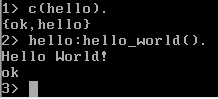
\includegraphics[width=0.5\textwidth]{konsoli2.png}
%\rotatebox{90}{\includegraphics[scale=.75]{esimerkki.pdf}}
\caption{Tuloste konsolilla}
\label{konsoli2}
%\end{center}
\end{figure}

Iteroinnissa C-kielest� tuttu tapa on mahdollinen

\begin{verbatim}
import std.stdio;

void main() {
  for(int i=0; i<10; i++) {
    writeln("Rivi: ", i);
  }
}
\end{verbatim}
Iteraatio voidaan tehd� my�s seuraavasti:
\begin{verbatim}
import std.stdio;

void main() {
  foreach(i; 0 .. 10) {
    writeln("Rivi: ", i);
  }
}
\end{verbatim}

ja tuloste n�ytt�� kuvan \ref{konsoli1} mukaiselta.
\begin{figure}[tbh]
%\begin{figure}[tbh] t= top, b = bottom, h=here
\begin{center}
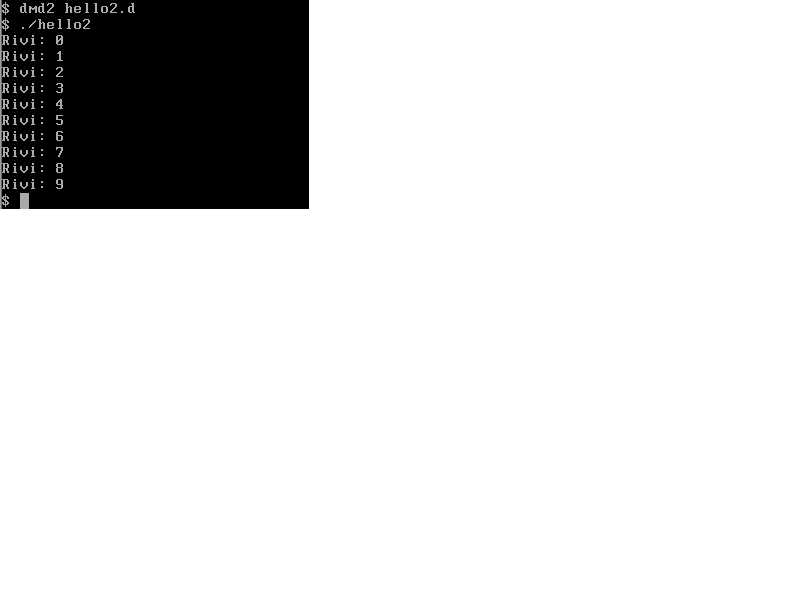
\includegraphics[width=1.0\textwidth]{konsoli1.jpg}
%\rotatebox{90}{\includegraphics[scale=.75]{esimerkki.pdf}}
\caption{Tuloste konsolilla}
\label{konsoli1}
\end{center}
\end{figure}

\section{Yhtenveto}
Yhteenvetona todettakoon, ett� D ja Erlang poikkeavat toisistaan...
\end{document}